%!TEX root = report.tex

\chapter{Études Préliminaires}

\section{Introduction du chapitre}

Dans ce chapitre on va procéder à la présentation des cas utilisateur de
notre système ainsi que l'identification des acteurs impliqués dans ces
cas. Puis on va décortiquer l’implémentation que nous proposons en citant
éventuellement nos motifs et intentions.

\section{Environnement de travail}

\subsection{Environnement de développement}%TODO
Plusieurs outils on était mise à contribution pour développer l'application, tant que sur le plan logiciel que matériel.

\subsubsection{Environnement Logiciel}
Voici une liste des outils logiciels utilisés pendant le développement de l'application.

\begin{description}

\item [Ubuntu 12.04] Système d'exploitation.\footnotemark[1]

\item [OpenJDK 6] \gls{jdk} version 6.\footnotemark[2]

\item [Eclipse Juno] Environnement de Développement Intégrer dans sa version \en{Service Release 2}.\footnotemark[3]

\item [\gls{adt} (plugin Eclipce)] Intégration des outils de développement fournit dans l'\gls{sdk} \android{}.\footnotemark[4]

\item [ObjectAid (plugin Eclipce)] Génération des diagrammes de classes.\footnotemark[5]

\item [PlantUML (plugin Eclipce)] Génération des diagrammes de séquences.\footnotemark[6]

\item [Git] Gestionnaire des versions\footnotemark[7].

\item [EGit (plugin Eclipse)] Intégration du gestionnaire de version.\footnotemark[8]

\item [Evolus Pencil] Génération de prototypes et des sketchs\footnotemark[9]
\end{description}

\footnotetext[1]{http://www.ubuntu.com}
\footnotetext[2]{http://openjdk.java.net}
\footnotetext[3]{http://www.eclipse.org}
\footnotetext[4]{https://developer.android.com/tools/sdk/eclipse-adt.html}
\footnotetext[5]{http://www.objectaid.com/}
\footnotetext[6]{http://plantuml.sourceforge.net/}
\footnotetext[7]{ttp://git-csm.com}
\footnotetext[8]{http://www.eclipse.org/egit/}
\footnotetext[9]{http://pencil.evolus.vn/}

\subsubsection{Environnement Matériel}

Le développement de l'application est fait avec une tablette Asus Nexus 7 (mise à jour à \android{} 4.2.2 \en{Jelly Bean}).

\section{Étude fonctionnel}

\subsection{Identification des acteurs}

Notre système interagit essentiellement avec trois acteurs différents:

\begin{description}

\item[Le médecin] C'est l'acteur principal de notre système.

\item[Le service web] Source des données à acheminer vers le médecin.

\item[Système d'exploitation] Communique à notre système les
informations recueillies des divers composants qui nous intéressent
(localisation GPS/Network, état de la connectivité, état de la
batterie).

\end{description}

\subsection{Cas d'utilisations}

On peut présenter les interactions fonctionnelles entre les acteurs gouverner par leurs besoins avec un diagramme des cas d'utilisations (figure \ref{fig:uml_usecase}).

\begin{figure}
\center
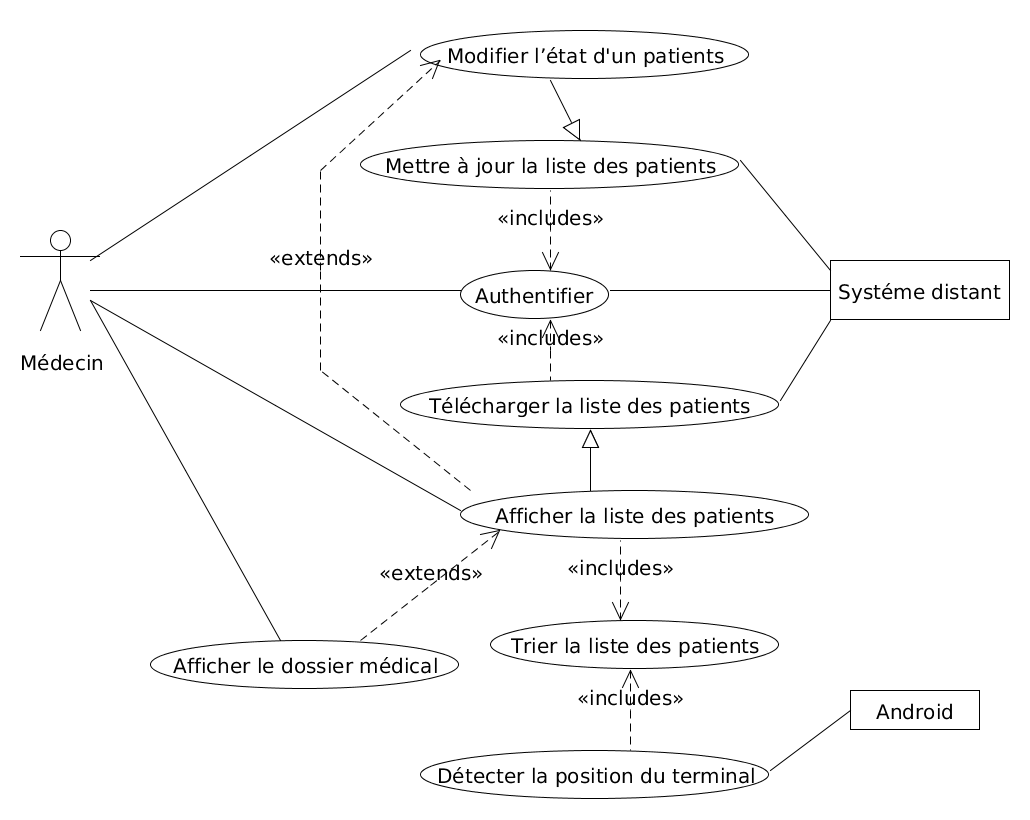
\includegraphics[width=0.8\textwidth]{diagrams/usecases}
\caption{Diagramme des cas d'utilisation \gls{uml} globale.}
\label{fig:uml_usecase}
\end{figure}

% \subsubsection{Cas: Authentifier}
% \subsubsection{Cas: Détecter la position du terminal}
% \subsubsection{Cas: Afficher la liste des patients}
% \subsubsection{Cas: Trier la liste des patients}
% \subsubsection{Cas: Modifier l’état d'un patients}
% \subsubsection{Cas: Afficher le dossier médical}
% \subsubsection{Cas: Télécharger la liste des patients}
% \subsubsection{Cas: Mettre à jour la liste des patients}

\subsection{Table de priorité}
